\chapter{Il sottosistema di I/O}

Il compito principale del sottosistema di \texttt{I/O} è quello di fornire un'interfaccia ai processi (utente e sistema) per l'accesso ai dispositivi di \texttt{I/O} tale che questa sia indipendente dal tipo di dispositivo e dalle sue caratteristiche fisiche. Il sottosistema di \texttt{I/O} deve quindi mettere in comunicazione l'\textit{hardware} ed il \textit{software} di \texttt{I/O} in modo che a prescindere dal tipo/modello di dispositivo, il sistema operativo possa fornire un'interfaccia uniforme e standardizzata per l'accesso ai dispositivi.

\section{Hardware di \texttt{I/O}}
    Il mercato libero ha portato alla proliferazione di dispositivi di \texttt{I/O} di ogni tipo e forma. Troviamo infatti dispositivi di memoria, di rete, di interazione con l'utente, di visualizzazione, di stampa, ecc. Possiamo inoltre distinguere i dispositivi dai controllori dei dispositivi, mentre i primi costituiscono la parte non elettronica del dispositivo, i secondi sono i circuiti elettronici che si occupano di gestire il dispositivo stesso.\newline
    Definiamo ora alcuni termini comuni a quasi tutti i dispositivi di \texttt{I/O}: Infatti ognuno di questi ha una porta che è il punto di connessione fisico tra il dispositivo e il computer. La porta è composta da un insieme di linee elettriche che possono essere utilizzate per inviare o ricevere dati. Le porte possono essere di tipo seriale o parallelo. Poi alcuni dispositivi funzionano su un \texttt{BUS} di sistema, che è un insieme di linee elettriche condivise da più dispositivi, il \texttt{BUS} può essere del tipo \textit{daisy chain} o condiviso. Infine ogni dispositivo ha un suo controllore che è un circuito elettronico che si occupa di gestire il dispositivo stesso e i segnali elettrici che provengono dalla porta. Il controllore è in grado di generare segnali di \texttt{I/O} e di interpretare i segnali provenienti dal dispositivo e dal sistema o da altri controllori.

    \subsubsection{Controllore dei dispositivi}
        Come già accennato, il controllore è un circuito elettronico che si occupa di gestire il dispositivo stesso e i segnali elettrici che provengono dalla porta. Questo è connesso al \texttt{BUS} di sistema, ed gli è associato un indirizzo univoco all'interno del sistema. Ogni controllore necessita di un registro/registri di stato, che contengono informazioni sullo stato del dispositivo e del controllore stesso (se ad esempio è pronto a ricevere dati o se ha terminato un'operazione di \texttt{I/O}). Inoltre ogni controllore ha un registro di controllo che viene usato per inviare comandi al dispositivo. Infine ogni controllore ha un \textit{buffer} per passare dai dati nel formato del \texttt{BUS} a quello del dispositivo e viceversa.
    \subsubsection{Comunicazione tra controllori e sistema}
        Per mettere in comunicazioni i registri del controllore con il resto del sistema operativo possono essere usate due principali tecniche ed una combinazione delle due. La prima è la \textit{memory-mapped \texttt{I/O}}, mentre la seconda è la \textit{\texttt{I/O} port-mapped}. 
            \paragraph{Memory-mapped \texttt{I/O}} 
                Nella \textit{memory-mapped \texttt{I/O}} i registri del controllore vengono mappati in un'area di memoria del sistema. In questo modo i processi possono inviare e ricevere comandi tramite le istruzione di accesso alla memoria. Ciò permette di scrivere dei \textit{driver} di \texttt{I/O} ad un livello più altro ed inoltre basta allocare la memoria in un'area che và al di fuori dell'area di memoria del sistema operativo per evitare problemi di sicurezza. 
            \paragraph{Port-mapped \texttt{I/O}}
                In questo caso l'accesso ai registri del controllore avviene tramite delle istruzioni specifiche per l'\texttt{I/O} che potenzialmente sono diverse per ogni controllore/dispositivo. In questo modo i registri del controllore non sono mappati in memoria il che risparmi un'area di memoria.
            \paragraph{Combinazione delle due}
                Un esempio di combinazione ibrida è l'architettura pentium dove i registri del controllore sono mappati tramite \textit{port-mapped \texttt{I/O}} e i \textit{buffer} coi dati sono mappati in memoria. In questo modo si risparmia memoria delle istruzioni di \texttt{I/O} e si possono usare le istruzioni di accesso alla memoria per accedere ai \textit{buffer}.
    \subsubsection{Accesso ai dispositivi}
        L'accesso ai dispositivi può avvenire in tre modi:
        \begin{itemize}
            \item \textit{Polling}
            \item \textit{Interrupt}
            \item \texttt{DMA} \textit{Direct Memory Access}
        \end{itemize}
        \paragraph{Polling}
            Il \textit{polling} è una tecnica di accesso ai dispositivi in cui il sistema operativo controlla periodicamente se il \textit{busy-bit} del registro di stato del controllore è attivo. Se il \textit{busy-bit} è impostato a \texttt{0} un nuovo comando può essere scritto nel registro di controllo del controllore e il \textit{command-ready-bit} viene impostato a \texttt{1}, viene quindi eseguita l'operazione di \texttt{I/O} e quando questa è terminata il \textit{busy-bit} viene impostato a \texttt{0}. Il \textit{polling} è una tecnica semplice da implementare ma causa un ciclo di attesa attiva che consuma risorse di sistema. 
        \paragraph{Interrupt}
            L'\textit{interrupt} è una tecnica di accesso ai dispositivi in cui il controllore invia un segnale al sistema operativo tramite una connessione fisica alla \texttt{CPU}. Quando il sistema operativo riceve il segnale di \texttt{I/O} interrompe l'esecuzione del processo corrente e salva il suo stato. Il sistema operativo esegue quindi il codice di gestione dell'\textit{interrupt} che si occupa di gestire l'operazione di \texttt{I/O} e ripristina lo stato del processo interrotto. Vanno però gestite delle situazioni dove il segnale di \textit{interrupt} arriva ma non può essere gestito immediatamente, ad esempio se si sta eseguendo un'operazione critica o se il sistema operativo è in uno stato di \textit{deadlock}. In questo caso il segnale di \textit{interrupt} deve essere messo in coda e gestito successivamente. Inoltre i segnali di \textit{interrupt} devono essere numerati in modo che la \texttt{CPU} esegua le corrette istruzioni di gestione dell'\textit{interrupt}. Infine \textit{interrupt} multipli devono essere gestiti tramite un sistema di priorità, in modo che i segnali più importanti vengano gestiti prima di quelli meno importanti.
            \begin{figure}[H]
                \centering
                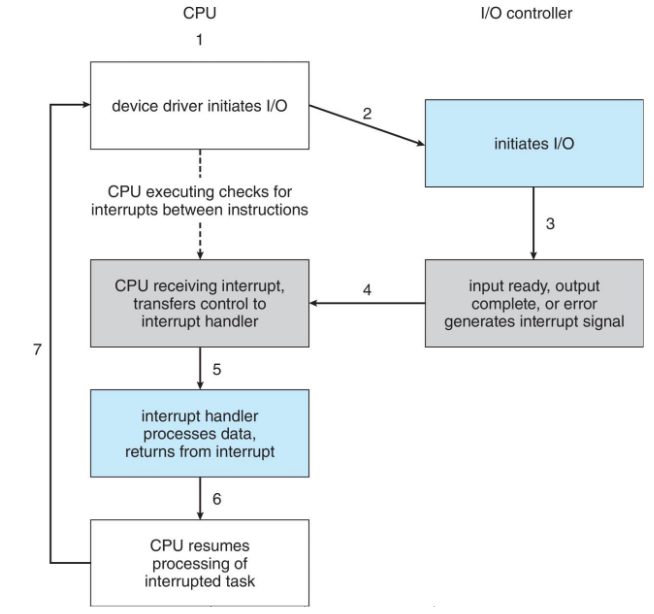
\includegraphics[width=0.5\textwidth]{14/interruptCycle.png}
                \caption{Ciclo della \texttt{CPU} per la gestione di \textit{interrupt}}
            \end{figure}
        \paragraph{DMA - \textit{Direct Memory Access}}
            Il \texttt{DMA} è una tecnica di accesso ai dispositivi ideata per grandi spostamenti di dati. Visto che usare la \texttt{CPU} per controllare solo pochi \texttt{byte} dal registro di stato del controllore è uno spreco di risorse, il \texttt{DMA} permette, tramite un \textit{hardware} dedicato, di trasferire i dati dalla memoria al dispositivo e viceversa senza l'intervento della \texttt{CPU}. Quando la \texttt{CPU} deve trasferire un grande blocco di dati, essa invia un comando al \texttt{DMA} contenete l'indirizzo di partenza dei blocchi di memoria da trasferire, l'indirizzo di destinazione, il numero di \texttt{byte} da trasferire e la direzione del trasferimento. Il \texttt{DMA} si occupa di gestire il trasferimento comunicando direttamente con il controller del dispositivo e con la memoria. Quando il trasferimento è terminato il \texttt{DMA} invia un segnale di \textit{interrupt} alla \texttt{CPU} per informarla che il trasferimento è terminato. Il \texttt{DMA} può essere usato in combinazione con il \textit{polling} o con gli \textit{interrupt}. Infatti il \texttt{DMA} può essere usato per trasferire i dati tra la memoria e il dispositivo, mentre la \texttt{CPU} può essere usata per gestire gli \textit{interrupt} e il \textit{polling}.
\section{Interfacce di \texttt{I/O}}
    Come già accennato, i dispositivi di \texttt{I/O} sono molto diversi tra loro e si differenziano per modalità di funzionamento, modalità di accesso, velocità di trasferimento, ecc. Per questo motivo è necessario usare un \textit{layer} aggiuntivo di software che si occupa di nascondere le differenze tra i vari dispositivi al \texttt{SO} e ai processi.\newline
    Questo \textit{layer} deve fornire una interfaccia comune ed uniforme per l'accesso ai dispositivi di \texttt{I/O} e deve essere in grado di gestire le differenze tra i vari dispositivi. Ecco quindi che introduciamo i \textit{driver}\newline
    Una prima grande distinzione è tra \textit{driver} per dispositivi a blocco e \textit{driver} per dispositivi a caratteri. I primi sono dispositivi nei quali è possibile memorizzare e trasferire i dati in blocchi di dimensione fissa, in questo genere di dispositivi è possibile leggere (\textit{read}), scrivere (\textit{write}) e cercare (\textit{seek}) i dati, questo è il caso di dischi rigidi, ecc\dots Questi dispositivi solitamente sono \textit{memory-mapped} e usano dei \textit{block-device drivers}.\newline
    I \textit{driver} per dispositivi a caratteri sono invece dispositivi nei quali i dati vengono trasferiti in modo sequenziale e non è possibile accedere ai dati in modo casuale. Quindi al posto di avere i comandi \textit{read}, \textit{write} e \textit{seek} abbiamo i comandi \textit{get} e \textit{put}. Questi dispositivi sono solitamente \textit{port-mapped} e usano dei \textit{character-device drivers}. Esempio di dispositivi a caratteri sono le stampanti, le porte seriali, i terminali, ecc\dots
\section{Software di \texttt{I/O}}
    La parte del \texttt{SO} che si occupa di gestire i dispositivi di \texttt{I/O} è chiamata \textit{I/O subsystem}. Questa parte deve essere indipendente dal dispositivo, la notazione deve essere uniforme e standardizzata, deve essere in grado di gestire gli errori e le varie opzioni di trasferimento dei dati. Il software è organizzato in quattro \textit{layer} principali:
    \begin{enumerate}
        \item Gestione degli \textit{interrupt}
        \item \textit{Device drivers}
        \item \texttt{SW} del \texttt{SO} indipendente dal dispositivo
        \item Programmi utente
    \end{enumerate}
    \paragraph{Gestione degli \textit{interrupt}}
        La gestione degli \textit{interrupt} è la parte del \texttt{SO} che si occupa di gestire gli \textit{interrupt} provenienti dai dispositivi di \texttt{I/O}. Gestisce inoltre le iterazioni coi controller dei dispositivi e la comunicazione con il \texttt{SW} del \texttt{SO} indipendente dal dispositivo. 
    \paragraph{\textit{Device drivers}}
        I \textit{device drivers} sono i programmi che si occupano di gestire i dispositivi di \texttt{I/O}. Questi programmi sono scritti dai produttori dei dispositivi e sono specifici per ogni dispositivo, prima di essere distribuiti questi sono firmati digitalmente dai produttori dei sistemi operativi. I \textit{device drivers} contengono tutto ciò che è \textit{device-dependent} e si occupano di gestire le differenze tra i vari dispositivi. I \textit{device drivers} sono spesso condivisi tra più dispositivi simili e sono tipicamente scritti in linguaggio macchina o in linguaggio \texttt{C}. 
    \paragraph{\texttt{SW} del \texttt{SO} indipendente dal dispositivo}
        Questa parte del \texttt{SO} si occupa di gestire le operazioni di \texttt{I/O} in modo uniforme e standardizzato. Inoltre deve gestire ed individuare i dispositivi collegati e gestirne i nomi. Inoltre deve proteggere tutte le operazioni di \texttt{I/O} dato che tutte le primitive di \texttt{I/O} sono privilegiate, và anche gestito il \textit{buffering} dei dati e la sincronizzazione tra i vari processi che accedono ai dispositivi di \texttt{I/O}, questo per gestire le differenti velocità, dimensioni e dimensioni di blocco dei vari dispositivi. Infine deve gestire gli errori, anche quelli \textit{device-dependent}, e l'allocazione ed il rilascio dei dispositivi.
        \subparagraph{Spooling} Lo \textit{spooling} è una tecnica di \texttt{I/O} che permette di gestire i dispositivi di \texttt{I/O} in modo efficiente. Questa tecnica consiste nel memorizzare i dati in un'area di memoria temporanea (chiamata \textit{spool}) prima di inviarli al dispositivo. In questo modo solo il processo \textit{spooler} deve gestire il dispositivo e gli altri processi possono continuare a lavorare senza dover aspettare il completamento dell'operazione di \texttt{I/O}. Inoltre lo \textit{spooling} permette di gestire i dispositivi in modo asincrono, ovvero i processi possono continuare a lavorare mentre i dati vengono trasferiti al dispositivo. Questa tecnica è molto utile per i dispositivi di \texttt{I/O} lenti come le stampanti o i dischi rigidi.
    \begin{figure}[H]
        \centering
        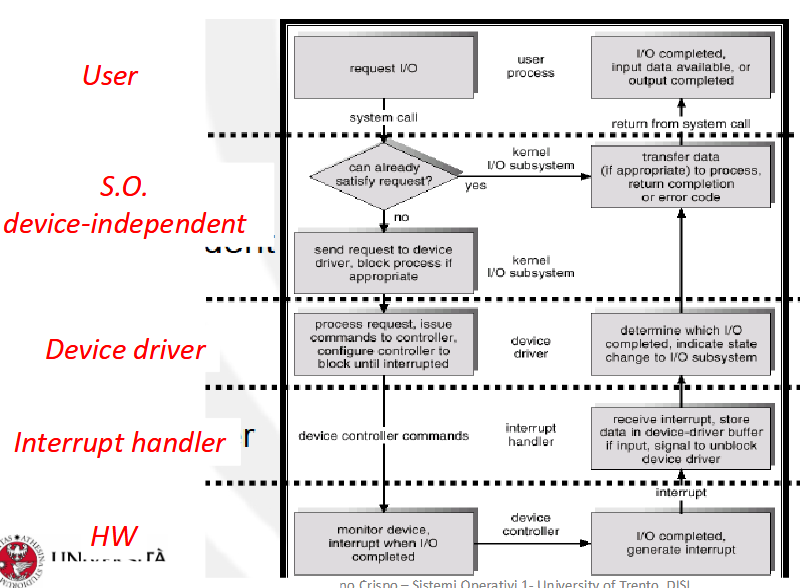
\includegraphics[width=0.7\textwidth]{14/ioSyscallCycle.png}
        \caption{Ciclo della \texttt{CPU} per la gestione di \texttt{I/O}}
    \end{figure}